%==============================================================================
%  Named Entity Recognition for Mizo
%  ACM TALLIP submission
%
%  Compile on Overleaf with pdfLaTeX:  pdflatex -> bibtex -> pdflatex x2
%
%  OPEN ITEMS are marked with  % TODO  throughout. Search for "TODO".
%==============================================================================
\documentclass[acmsmall,screen,review]{acmart}

\acmJournal{TALLIP}
\acmVolume{0}
\acmNumber{0}
\acmArticle{0}
\acmYear{2026}
\acmMonth{1}
\setcopyright{acmlicensed}

\usepackage{enumitem}
\setlength{\headheight}{19pt}
\addtolength{\topmargin}{-6pt}
\usepackage{amsmath}
\usepackage{tikz}
\usetikzlibrary{arrows.meta, positioning}

%------------------------------------------------------------------ CCS
\begin{CCSXML}
<ccs2012>
 <concept>
  <concept_id>10010147.10010178.10010179.10003352</concept_id>
  <concept_desc>Computing methodologies~Information extraction</concept_desc>
  <concept_significance>500</concept_significance>
 </concept>
 <concept>
  <concept_id>10010147.10010178.10010179.10010181</concept_id>
  <concept_desc>Computing methodologies~Machine translation</concept_desc>
  <concept_significance>500</concept_significance>
 </concept>
 <concept>
  <concept_id>10010147.10010257.10010258.10010259</concept_id>
  <concept_desc>Computing methodologies~Language resources</concept_desc>
  <concept_significance>300</concept_significance>
 </concept>
</ccs2012>
\end{CCSXML}
\ccsdesc[500]{Computing methodologies~Information extraction}
\ccsdesc[500]{Computing methodologies~Machine translation}
\ccsdesc[300]{Computing methodologies~Language resources}

\keywords{Named entity recognition, low-resource languages, Mizo, Tibeto-Burman,
Indic NLP, cross-lingual annotation projection, silver-standard corpus,
XLM-RoBERTa, neural machine translation, entity-aware translation}

\title{Named Entity Recognition for Mizo: A Silver-Standard Corpus via
       Cross-Lingual Projection and Its Effect on Machine Translation}

%------------------------------------------------------------------ Authors
\author{Thangkhanhau Haulai}
\authornote{Corresponding author.}
\orcid{0000-0001-7154-5364}
\email{tka@gsc.edu.in}
\affiliation{%
  \institution{Department of Computer Science, Government Serchhip College}
  \city{Serchhip}
  \state{Mizoram}
  \country{India}
}

\author{Jamal Hussain}
\orcid{0000-0001-5553-3654}
\email{jamal.mzu@gmail.com}
\affiliation{%
  \institution{Department of Mathematics \& Computer Science, Mizoram University}
  \city{Aizawl}
  \state{Mizoram}
  \country{India}
}

\author{MS Dawngliani}
\orcid{0000-0002-5808-2438}
\email{adawngi@gzrsc.edu.in}
\affiliation{%
  \institution{Department of Computer Science, Govt.\ Zirtiri Residential Science College}
  \city{Aizawl}
  \state{Mizoram}
  \country{India}
}

\author{Verónica Vargas-Alejo}
\orcid{0000-0002-7431-0568}
\email{veronica.vargas@academicos.udg.mx}
\affiliation{%
  \institution{CUCEI, Universidad de Guadalajara}
  \city{Guadalajara}
  \state{Jalisco}
  \country{Mexico}
}

\renewcommand{\shortauthors}{Haulai et al.}

%==============================================================================
\begin{document}

\begin{abstract}
Mizo, a Tibeto-Burman language of the Kuki-Chin branch spoken across northeast
India, has until recently had no annotated data for named entity recognition.
The gold-standard resources that now exist are necessarily small, and the
language remains without a gazetteer, a morphological analyzer, or coverage in
the pretraining data of standard multilingual encoders. This paper contributes
a resource at a different point on the size-quality trade-off: a
silver-standard corpus of 441,178 Mizo sentences carrying 590,655 entity
annotations over eleven types, built by projecting spaCy-detected English
entities across a Mizo--English parallel corpus of 1,357,838 sentence pairs.
The projection matcher is deliberately morphology-aware, and we quantify why
that matters: on a held-out subset, exact string matching recovers 4.14\% of
English entities, while adding suffix-aware matching for Mizo's productive case
markers raises recovery to 41.91\%, a tenfold gain. Eight rounds of inspection
over random samples yielded a rule set that corrected 100,237 labels.
Fine-tuning XLM-RoBERTa on this corpus reaches 97.84\% token accuracy and a
micro-averaged $F_1$ of 0.8529 on a held-out silver test set, despite Mizo's
absence from the encoder's pretraining. Per-type $F_1$ tracks annotation
frequency closely (Spearman $\rho = 0.75$, $p = 0.008$), locating the binding
constraint in data rather than in architecture. A second experiment inserts
entity markup into the source side of a Mizo-to-English translation system and
finds a small but consistent gain of $+0.33$ BLEU and $+0.24$ ChrF (bootstrap
$p = 0.001$, 95\% CI $[+0.136, +0.530]$). Because that markup is drawn from the
corrected projection rather than from the recognizer, the figure is an upper
bound on what a deployed pipeline would deliver. We report throughout that all
labels, training and test alike, are silver-standard, so the recognition scores
measure agreement with the projection rather than accuracy against human
judgment.
\end{abstract}

\maketitle

%==============================================================================
\section{Introduction}
\label{sec:intro}

Named entity recognition---locating and classifying mentions of persons, places,
organizations, and related categories---sits early in most language processing
pipelines and feeds question answering, information retrieval, relation
extraction, and machine translation. For a small number of languages, large
manually annotated corpora and strong pretrained encoders have brought the task
close to human agreement. For most of the world's languages the annotated data
that would make any of that reachable simply does not exist.

Mizo (\textit{Mizo tawng}, historically \textit{Lushai}) is a scheduled language
of India in the Kuki-Chin branch of Tibeto-Burman, the principal language of
Mizoram, and a lingua franca across much of the northeast Indian hill region.%
\footnote{TODO: cite the 2011 Census of India language tables for the speaker
population before submission.}
Computational work on Mizo has grown noticeably in the last decade, from early
resource building and part-of-speech tagging \citep{pakray2015mizopos} through
translation systems \citep{khenglawt2024mizomt} to a language-specific
pretrained encoder \citep{lalramhluna2024mizbert}. Entity recognition has moved
more slowly. \citet{bentham2016mizoner} identified rules for Mizo entity classes
over a small news sample, and \citet{ghosh2025mizokhasi} recently released
human-annotated gold-standard datasets for Mizo and Khasi covering
part-of-speech tagging, entity recognition, and keyword identification, together
with a synthetic pipeline that translates from Hindi and aligns across
languages. Gold annotation is the right foundation and is what the field needed
first. It is also, unavoidably, expensive: the pool of annotators fluent in Mizo
and trained in the task is very small, which bounds how large such a resource
can be.

This paper occupies the complementary position. Rather than annotate carefully
at small scale, we project automatically at large scale and are explicit about
the cost in label quality. Cross-lingual annotation projection transfers labels
from a well-resourced language to a target language through parallel text and
has been applied across a widening range of low-resource settings
\citep{hedderich2021,adelani2022masakhaner,mhaske2023naamapadam}. The trade is
precision for volume: the result is silver-standard, noisy but large. Our route
differs from that of \citet{ghosh2025mizokhasi} in its pivot---English rather
than Hindi---and in its matching strategy, which is built around Mizo
morphology rather than around a neural aligner.

Four contributions follow.

\begin{enumerate}[leftmargin=*,label=(\arabic*)]
  \item \textbf{A large silver-standard Mizo entity corpus.} 441,178 sentences
        carrying 590,655 annotations across eleven types, larger than existing
        Mizo entity resources by orders of magnitude, with retention reported at
        every stage of construction.
  \item \textbf{A quantified account of what morphology-aware projection buys.}
        On a held-out subset, exact matching recovers 4.14\% of English entities
        and suffix-aware matching 41.91\%. Projection papers commonly report
        corpus size and omit recovery; the tenfold difference here is the
        substance of the method for a language that suffixes proper nouns as
        freely as Mizo does.
  \item \textbf{A neural entity recognizer for Mizo trained at scale.}
        Fine-tuned XLM-RoBERTa reaching 97.84\% token accuracy and micro-$F_1$
        0.8529, with per-type analysis showing performance governed by
        annotation frequency rather than by linguistic difficulty.
  \item \textbf{An upper bound on the value of entity markup for Mizo--English
        translation.} Source-side markup yields $+0.33$ BLEU and $+0.24$ ChrF,
        statistically reliable in direction, modest in size, and concentrated in
        the frequent types. We are not aware of prior work testing entity markup
        for this language pair.
\end{enumerate}

Two cautions belong here rather than buried in a closing section. First, every
label in this work is silver-standard. The test partition was produced by the
same projection pipeline as the training partition, so the recognition scores
measure agreement with the projection, not accuracy against human annotation;
the true figure is unknown and is likely lower.
Section~\ref{sec:limitations} treats this as the principal limitation and
Section~\ref{sec:discussion:calibration} explains what would fix it. Second, the
translation experiment injects markup taken from the corrected projection, not
predictions from the recognizer. It measures what entity markup is worth when
the markup is already consistent with the corpus the translation model was
trained on, which bounds from above what a recognizer-driven pipeline would
achieve.

Section~\ref{sec:mizo} describes the language properties that shape the task and
Section~\ref{sec:related} situates the work. Sections~\ref{sec:corpus}
and~\ref{sec:tagset} cover corpus construction and the annotation scheme.
Sections~\ref{sec:model} and~\ref{sec:nereval} present the recognizer and its
evaluation, Sections~\ref{sec:mt} and~\ref{sec:mtresults} the translation
experiment. Section~\ref{sec:discussion} discusses,
Section~\ref{sec:limitations} states limitations, and
Section~\ref{sec:conclusion} concludes.

%==============================================================================
\section{The Mizo Language}
\label{sec:mizo}

Mizo belongs to the Kuki-Chin branch of Tibeto-Burman, alongside languages such
as Tenyidie \citep{angami2025tenyidie} and Bodo \citep{narzary2024bodo} whose
entity resources have appeared only recently. It is the sole official language
of Mizoram.

\paragraph{Morphology.}
Mizo marks case through postpositional suffixes attaching directly to the noun,
among them the locative \textit{-ah}, the agentive and instrumental \textit{-in},
and \textit{-a} and \textit{-an}. These attach to named entities as readily as
to common nouns, so a single entity surfaces in several forms according to its
syntactic role: \textit{Aizawl} appears as \textit{Aizawlah}, \textit{Liana} as
\textit{Liana-an}. Any projection method comparing surface forms alone will miss
every inflected variant, which is the motivation for the matcher of
Section~\ref{sec:corpus:projection}.

\paragraph{Syntax and script.}
Mizo is verb-final with head-final nominal structure and no articles, giving
systematic word-order divergence from English. It is written in the Latin
script, which removes the transliteration barrier that complicates projection
into abugida or logographic systems and makes direct string comparison viable.

\paragraph{Why entities are hard here.}
Four properties compound. Mizo personal names are drawn from the language's own
lexicon and are not cognate with English or Hindi names, so cross-lingual
lexical overlap is low. Productive suffixation multiplies surface forms per
entity. No gazetteer or entity lexicon exists to fall back on. And Mizo is
absent from the pretraining corpora of the standard multilingual encoders, so a
model cannot draw on entity knowledge acquired during pretraining. A further
difficulty is internal ambiguity: many Mizo personal names are formally
indistinguishable from place names, a confusion that
Section~\ref{sec:nereval:errors} shows the recognizer inheriting directly from
the projection.

%==============================================================================
\section{Related Work}
\label{sec:related}

\subsection{Computational Resources for Mizo}
\label{sec:related:mizo}

Work on Mizo began with resource construction and part-of-speech tagging
\citep{pakray2015mizopos} and rule identification for entity classes over a
small news sample \citep{bentham2016mizoner}. Translation has attracted the most
sustained attention, with data augmentation and language modeling applied to the
English--Mizo direction \citep{khenglawt2024mizomt}, and parallel corpus
construction reported separately \citep{dawngliani2023mizocorpus}. More
recently, \citet{lalramhluna2024mizbert} pretrained MizBERT, a Mizo-specific
BERT trained on text collected from online sources and evaluated by masked
language modeling accuracy and perplexity.

The most direct predecessor to the present work is
\citet{ghosh2025mizokhasi}, who release human-annotated gold-standard datasets
for Mizo and Khasi spanning part-of-speech tagging, entity recognition, and
keyword identification, with custom annotation guidelines for the entity task,
and who additionally explore synthetic entity data generated by translating from
Hindi and aligning across languages. Their contribution is annotation quality;
ours is scale and a different pivot language. The two are complementary in a
concrete sense: a gold test set of the kind they construct is precisely what
would calibrate the silver-standard evaluation reported here, and we say so in
Section~\ref{sec:limitations} rather than claiming our numbers are already
comparable to theirs.

We do not claim priority for Mizo entity recognition. What we claim is a
resource roughly three orders of magnitude larger than what gold annotation has
so far been able to produce for this language, a quantified account of what
morphology-aware projection contributes, and the first evaluation of entity
markup for Mizo--English translation.

\subsection{Entity Recognition for Low-Resource Languages}
\label{sec:related:lowresource}

Two strategies dominate. Model transfer applies a multilingual encoder to the
target language with no target-language training data. Data transfer generates
target-language training examples from parallel text or translation.
\citet{hedderich2021} survey both and find that data quality, domain match, and
linguistic distance between source and target govern how well either works.

MasakhaNER \citep{adelani2022masakhaner} provides annotated data for 21 African
languages and shows that fine-tuning on even a small gold corpus beats zero-shot
transfer consistently, with augmentation partly compensating when gold data is
scarce. For Indic languages, Naamapadam \citep{mhaske2023naamapadam} is the
largest systematic effort, projecting English entities across the Samanantar
parallel corpus for 11 languages. Our method is closest to Naamapadam in spirit.
Mizo is not among its languages, and our adaptation is to morphology rather than
to script or alignment. MulDA \citep{liu2021mulda} takes the complementary route
of translating labeled high-resource data, and its finding that translated
silver data competes with limited gold data supports the general viability of
silver-standard training.

\subsection{Cross-Lingual Annotation Projection}
\label{sec:related:projection}

Projection transfers labels across parallel text using word alignments. Quality
depends on alignment accuracy, morphological divergence, and the frequency of
the projected type. Several methods improve substantially on naive projection.
CROP \citep{yang2022crop} recasts projection as labeled-sequence translation.
T-Projection \citep{garcia2022tprojection} generates candidate annotations with
a text-to-text model and ranks them by translation probability. TransFusion
\citep{chen2023transfusion} annotates in a high-resource language and fuses the
annotations back. CoLaDa \citep{colada2023} attacks projection noise through
collaborative label denoising, and constrained decoding
\citep{le2024constrained} avoids the translation degradation that marker
insertion can cause.

Our matcher is simpler than all of these, and the reason is availability rather
than preference. No Mizo word aligner exists. No Mizo--English translation model
of sufficient quality exists for the back-translation step CROP and TransFusion
require. What Mizo does offer is a small, regular, productive suffix inventory,
which makes rule-based stripping effective at a fraction of the cost. We expect
T-Projection or constrained decoding to raise recall once the enabling models
exist for Mizo; frustratingly easy label projection
\citep{wu2022frustratingly} is attractive in the interim because it needs only a
parallel corpus and a source-language tagger.

\subsection{Tibeto-Burman and Indic Neighbors}
\label{sec:related:indic}

\citet{angami2025tenyidie} present an entity corpus for Tenyidie with CRF,
BiLSTM, and BERT baselines; their finding that transformer models win even on
small corpora matches what we observe. \citet{narzary2024bodo} describe a Bodo
dataset with deep learning baselines, and \citet{islam2025nagamese} release a
Nagamese corpus with MEMM and CRF baselines. Together these establish that the
task is tractable across the region given annotated data. Mizo shares the
relevant morphological properties with Tenyidie and Bodo.

\subsection{Multilingual Encoders for Sequence Labeling}
\label{sec:related:transformers}

Multilingual BERT \citep{devlin2019bert} and XLM-RoBERTa
\citep{conneau2020xlmr} changed low-resource entity recognition by supplying
shared representations across a hundred languages. XLM-RoBERTa outperforms mBERT
across cross-lingual transfer benchmarks and shows non-trivial performance even
on languages absent from its pretraining, apparently by learning subword
patterns that generalize across families. Mizo is one such absent language, and
its Latin script means its subword inventory overlaps considerably with
languages the model did see.

We selected XLM-RoBERTa on the strength of the low-resource results in
\citet{adelani2022masakhaner} and \citet{mhaske2023naamapadam}. We note plainly
that MizBERT \citep{lalramhluna2024mizbert} is now available and is the natural
comparison point for a Mizo-specific encoder; it postdates the experiments
reported here and Section~\ref{sec:limitations} records its absence as a
limitation rather than arguing it away.

\subsection{Entity-Aware Neural Machine Translation}
\label{sec:related:entitymt}

Entities are hard for translation systems because they are individually rare,
frequently out of vocabulary, and require consistent transliteration that a
general model may lack the data to learn. \citet{zeng2023extract} prefix
candidate entity translations to the decoder input and reduce entity error rates
on English-to-Chinese and English-to-Russian. \citet{nguyen2025multitask}
optimize translation and entity objectives jointly. For South Asian languages,
\citet{ranathunga2024parallel} show that entity-annotated parallel corpora
improve low-resource translation directly, linking resource creation to
downstream benefit in a setting close to ours.

The integration we test is the simplest of these: mark the spans in the source
string, then translate. It requires no architectural change and works with any
black-box system.

%==============================================================================
\section{Corpus Construction}
\label{sec:corpus}

\subsection{Source Data and English-Side Detection}
\label{sec:corpus:source}

Construction starts from a Mizo--English parallel corpus of 1,357,838 sentence
pairs assembled for earlier work on Mizo--English translation
\citep{dawngliani2023mizocorpus}. Entities were detected on the English side
using spaCy's \texttt{en\_core\_web\_sm} model \citep{honnibal2020spacy}, which
annotates against the OntoNotes~5 inventory \citep{weischedel2013ontonotes}.
Pairs whose English side contained no entity of a retained type were discarded,
leaving 640,146 pairs, or 47.1\% of the original. This both reduces processing
cost and concentrates the corpus on entity-bearing text;
Section~\ref{sec:limitations} records what it costs.

\subsection{Projection}
\label{sec:corpus:projection}

Let $(s^{\mathrm{en}}, s^{\mathrm{mz}})$ be an aligned sentence pair and let
$\mathcal{E}(s^{\mathrm{en}}) = \{(e_i, T_i)\}_{i=1}^{k}$ be the entities
detected on the English side, each a surface string $e_i$ with type $T_i$.
Writing $\mathcal{T}(s^{\mathrm{mz}})$ for the token sequence of the Mizo
sentence and $\sigma(\cdot)$ for the suffix-stripping operator, the matcher
accepts a Mizo token $t$ as a realization of $e_i$ when

\begin{equation}
\label{eq:match}
\mathrm{match}(t, e_i) =
\begin{cases}
1 & \text{if } \mathrm{lower}(t) = \mathrm{lower}(e_i), \\[2pt]
1 & \text{if } \mathrm{lower}(\sigma(t)) = \mathrm{lower}(e_i), \\[2pt]
0 & \text{otherwise,}
\end{cases}
\end{equation}

where $\sigma$ removes one element of the suffix inventory
$\Sigma = \{\textit{-ah}, \textit{-in}, \textit{-a}, \textit{-an}, \ldots\}$
described in Section~\ref{sec:mizo}, and hyphens are treated as segment
boundaries so that the common orthographic pattern \textit{Liana-an} resolves
correctly. The first clause of Equation~\eqref{eq:match} is exact matching; the
second is the morphology-aware extension. Multi-token entities are matched
greedily longest-first so that nested candidates resolve to the longer span. The
projected annotation set for the Mizo sentence is then

\begin{equation}
\label{eq:project}
\mathcal{E}(s^{\mathrm{mz}}) =
\bigl\{ (\mathrm{span}(t), T_i) \;:\; t \in \mathcal{T}(s^{\mathrm{mz}}),\;
(e_i,T_i) \in \mathcal{E}(s^{\mathrm{en}}),\;
\mathrm{match}(t,e_i) = 1 \bigr\}.
\end{equation}

Table~\ref{tab:projection_recovery} reports what each clause recovers, measured
on a held-out subset of 3,829 sentence pairs containing 5,142 English entities.
Exact matching alone finds 213. Adding the suffix-aware clause raises this to
2,155, a tenfold increase, and lifts the proportion of sentences receiving at
least one projected entity from 4.8\% to 47.3\%.

For a language whose case system attaches to proper nouns as freely as Mizo's
does, this is not a refinement of the method but its substance. The figure also
sets an expectation: recovery stops well short of half, so the corpus is large
because the underlying parallel corpus is large, not because the matcher is
thorough.

\begin{table}[htbp]
\centering
\caption{Entity recovery by matching clause, measured on 3,829 held-out
sentence pairs containing 5,142 English entities.}
\label{tab:projection_recovery}
\begin{tabular}{lrrrr}
\hline
\textbf{Matching clause} & \textbf{Entities} & \textbf{Recovery} & \multicolumn{2}{c}{\textbf{Sentences with $\geq$1 match}} \\
                         & \textbf{recovered} & \textbf{(\%)}    & \textbf{count} & \textbf{(\%)} \\
\hline
Exact only            &   213 &  4.14 &   184 &  4.8 \\
Exact + suffix-aware  & 2,155 & 41.91 & 1,811 & 47.3 \\
\hline
\end{tabular}
\end{table}

\subsection{Correction and Deduplication}
\label{sec:corpus:correction}

Projection over the filtered corpus produced annotations for 442,180 sentences,
69.1\% of those submitted, carrying 592,361 spans. The remainder received no
projected entity and were dropped.

The raw projection is noisy in ways visible on inspection. Mizo personal names
were frequently assigned \texttt{GPE} or \texttt{ORG} rather than
\texttt{PERSON}, either because the English-side model had itself mislabeled
them or because the matcher had attached a label to the wrong span. Correction
proceeded in eight rounds. Each round drew a random sample of 20 to 30 annotated
sentences for manual inspection, and errors found were generalized into
label-correction rules applied across the whole corpus. The rule set grew from
31 rules to 62. The final pass corrected 100,237 labels and removed 952 spurious
spans; sentences left with no remaining entity were dropped.

We describe this as rule-based correction guided by manual inspection, and not
as manual verification, because fewer than 250 sentences were ever read by a
human. Section~\ref{sec:discussion:projection} reports what inspection of the
final rounds still turns up.

Exact-duplicate sentences were then removed on a normalized form ignoring case,
punctuation, and repeated whitespace, eliminating 562 sentences.
Figure~\ref{fig:pipeline} summarizes the sequence and Table~\ref{tab:funnel}
gives the counts.

\begin{figure}[htbp]
\centering
\begin{tikzpicture}[
  node distance=6mm,
  box/.style={draw, rounded corners=2pt, align=center, inner sep=4pt,
              font=\small, minimum height=8mm, text width=34mm},
  arr/.style={-{Latex[length=2mm]}, thick}
]
\node[box] (a) {Parallel corpus\\\textbf{1,357,838} pairs};
\node[box, below=of a] (b) {English entity filter\\\textbf{640,146} (47.1\%)};
\node[box, below=of b] (c) {Projection to Mizo\\\textbf{442,180} (69.1\%)};
\node[box, below=of c] (d) {Rule correction\\8 rounds, 62 rules};
\node[box, below=of d] (e) {Deduplication\\\textbf{441,178} sentences};
\draw[arr] (a) -- (b);
\draw[arr] (b) -- (c);
\draw[arr] (c) -- (d);
\draw[arr] (d) -- (e);
\node[right=4mm of b, font=\scriptsize, align=left, text width=52mm]
  {spaCy \texttt{en\_core\_web\_sm}; pairs with no English entity discarded};
\node[right=4mm of c, font=\scriptsize, align=left, text width=52mm]
  {Equation~\eqref{eq:match}: exact + suffix-aware; sentences with no projected entity discarded};
\node[right=4mm of d, font=\scriptsize, align=left, text width=52mm]
  {100,237 labels corrected, 952 spans removed};
\node[right=4mm of e, font=\scriptsize, align=left, text width=52mm]
  {562 duplicates removed; 590,655 entities remain};
\end{tikzpicture}
\caption{Corpus construction pipeline with retention at each stage.}
\Description{Flow chart with five stacked boxes showing corpus construction. The parallel corpus of 1,357,838 sentence pairs is filtered to 640,146 pairs containing an English entity, projected to 442,180 Mizo sentences, corrected over eight rule rounds, and deduplicated to a final 441,178 sentences carrying 590,655 entities.}
\label{fig:pipeline}
\end{figure}

\begin{table}[htbp]
\centering
\caption{Sentence counts through corpus construction.}
\label{tab:funnel}
\begin{tabular}{lrr}
\hline
\textbf{Stage} & \textbf{Sentences} & \textbf{Retained (\%)} \\
\hline
Parallel corpus                         & 1,357,838 & --- \\
Contains an English entity              &   640,146 & 47.1 \\
At least one entity projected to Mizo   &   442,180 & 69.1 \\
After rule correction and deduplication &   441,178 & 99.8 \\
\hline
\end{tabular}
\end{table}

\subsection{Corpus Statistics}
\label{sec:corpus:stats}

The final corpus holds 441,178 sentences and 590,655 annotations, an average of
1.34 entities per sentence and at most 8 in any one sentence. Sentences run from
4 to 33 tokens, mean 11.3 and median 11, with the 95th percentile at 19 tokens
and the 99th at 26. Table~\ref{tab:entity_distribution} gives the distribution
across types.

The distribution is heavily skewed. \texttt{PERSON}, \texttt{GPE}, and
\texttt{ORG} account for 92.8\% of all annotations, while \texttt{EVENT} and
\texttt{LAW} together account for less than a quarter of one percent. This is
not an artifact of the matcher. It reflects both what appears in the underlying
text and what the English-side model detects reliably, and it governs the
per-type results of Section~\ref{sec:nereval:perentity}.

\begin{table}[htbp]
\centering
\caption{Entity type distribution in the final corpus.}
\label{tab:entity_distribution}
\begin{tabular}{lrr}
\hline
\textbf{Entity type} & \textbf{Count} & \textbf{Share (\%)} \\
\hline
PERSON        & 326,997 & 55.36 \\
GPE           & 116,492 & 19.72 \\
ORG           & 104,472 & 17.69 \\
NORP          &  19,723 &  3.34 \\
LOC           &   6,857 &  1.16 \\
LANGUAGE      &   4,655 &  0.79 \\
WORK\_OF\_ART &   3,886 &  0.66 \\
FAC           &   3,174 &  0.54 \\
PRODUCT       &   2,934 &  0.50 \\
EVENT         &     884 &  0.15 \\
LAW           &     581 &  0.10 \\
\hline
\textbf{Total} & \textbf{590,655} & \textbf{100.00} \\
\hline
\end{tabular}
\end{table}

%==============================================================================
\section{Annotation Scheme}
\label{sec:tagset}

\subsection{Entity Types}
\label{sec:tagset:types}

We retain eleven types from the OntoNotes~5 inventory used by the English model:
\texttt{PERSON} for individuals and fictional characters; \texttt{ORG} for
institutions, companies, and government bodies; \texttt{GPE} for countries,
states, and cities; \texttt{LOC} for non-political locations such as rivers,
mountains, and regions; \texttt{NORP} for nationalities, religious groups, and
political affiliations; \texttt{FAC} for buildings, airports, and
infrastructure; \texttt{LAW} for named legal instruments; \texttt{EVENT} for
named events; \texttt{PRODUCT} for manufactured or branded items;
\texttt{WORK\_OF\_ART} for titles of books, songs, films, and artworks; and
\texttt{LANGUAGE} for names of languages.

Numeric and temporal categories such as \texttt{DATE}, \texttt{CARDINAL}, and
\texttt{ORDINAL} were dropped. They project almost trivially through exact
matching, since numerals are typically identical on both sides, and retaining
them would inflate the recovery figures of
Table~\ref{tab:projection_recovery} without testing the part of the method that
matters. Retaining eleven types rather than collapsing to a coarser scheme costs
accuracy on the rare categories; we keep them because the finer distinctions are
what a downstream consumer needs, and because collapsing would hide the sparsity
problem rather than solve it.

\subsection{Format and Encoding}
\label{sec:tagset:format}

Annotations are stored as character offsets with labels in JSON Lines, one
sentence per line, each record holding the Mizo sentence, its spans, and the
English sentence it was projected from. For model training the spans are
converted to BIO encoding \citep{ramshaw1995chunking}, giving
$2 \times 11 + 1 = 23$ labels. Table~\ref{tab:bio_example} shows a sentence in
both forms.

\begin{table}[htbp]
\centering
\caption{BIO encoding of \textit{Alvin chuan Cairo kawtthler atangin Cindy a
chhan chhuak a.} (``Alvin rescued Cindy from the streets of Cairo.'')}
\label{tab:bio_example}
\small
\begin{tabular}{llcll}
\hline
\textbf{Token} & \textbf{Tag} & \hspace{6mm} & \textbf{Token} & \textbf{Tag} \\
\hline
Alvin     & B-PERSON & & Cindy  & B-PERSON \\
chuan     & O        & & a      & O \\
Cairo     & B-GPE    & & chhan  & O \\
kawtthler & O        & & chhuak & O \\
atangin   & O        & & a.     & O \\
\hline
\end{tabular}
\end{table}

%==============================================================================
\section{The Recognition Model}
\label{sec:model}

\subsection{Architecture and Objective}
\label{sec:model:arch}

We fine-tune XLM-RoBERTa\textsubscript{base} \citep{conneau2020xlmr} with a
linear token classification head over the 23 BIO labels. For an input sequence
$x = (x_1, \ldots, x_n)$ of subword tokens, the encoder produces contextual
representations $h_i \in \mathbb{R}^{d}$ with $d = 768$, and the head assigns

\begin{equation}
\label{eq:softmax}
p(y_i = c \mid x) = \frac{\exp\bigl(w_c^{\top} h_i + b_c\bigr)}
                         {\sum_{c' \in \mathcal{C}} \exp\bigl(w_{c'}^{\top} h_i + b_{c'}\bigr)},
\qquad |\mathcal{C}| = 23 .
\end{equation}

Training minimizes token-level cross-entropy over the first subword of each
word, with continuation subwords and padding masked out of the loss:

\begin{equation}
\label{eq:loss}
\mathcal{L} = - \frac{1}{|\mathcal{M}|}
              \sum_{i \in \mathcal{M}} \log p\bigl(y_i = y_i^{\ast} \mid x\bigr),
\end{equation}

where $\mathcal{M}$ indexes the unmasked positions and $y_i^{\ast}$ is the
projected label. No conditional random field layer is used; decoding takes the
argmax at each position independently.

Mizo is absent from the encoder's pretraining corpus, so whatever the encoder
contributes comes from cross-lingual transfer rather than familiarity with the
language. The model was not adapted through continued pretraining on unlabeled
Mizo text, which remains an obvious next step now that a Mizo-specific encoder
exists \citep{lalramhluna2024mizbert}.

\subsection{Data Splits and Training}
\label{sec:model:training}

The corpus was split 80/10/10 at the sentence level with a fixed seed, giving
352,941 training, 44,118 development, and 44,118 test sentences. One record was
dropped during BIO conversion for a null entity string, so the split covers
441,177 sentences.

Table~\ref{tab:training_config} lists the configuration. Training ran for five
epochs on a single consumer GPU and the checkpoint with best development $F_1$
was retained.

\begin{table}[htbp]
\centering
\caption{Recognition model training configuration.}
\label{tab:training_config}
\begin{tabular}{ll}
\hline
\textbf{Parameter} & \textbf{Value} \\
\hline
Model                   & \texttt{xlm-roberta-base} \\
Maximum sequence length & 64 subword tokens \\
Epochs                  & 5 \\
Learning rate           & $2 \times 10^{-5}$ \\
Optimizer               & AdamW \citep{loshchilov2019adamw} \\
Batch size              & 32, gradient accumulation 2 (effective 64) \\
Weight decay            & 0.01 \\
Warmup ratio            & 0.1 \\
Mixed precision         & fp16 \\
Checkpoint selection    & best development micro-$F_1$ \\
Training / dev / test   & 352,941 / 44,118 / 44,118 sentences \\
Hardware                & NVIDIA RTX 3050 Laptop, 4\,GB \\
Training time           & 15.01 hours \\
\hline
\end{tabular}
\end{table}

\subsection{Evaluation Protocol}
\label{sec:model:eval}

We report entity-level precision, recall, and $F_1$ under exact span matching
using \texttt{seqeval}. Writing $\mathrm{TP}_c$, $\mathrm{FP}_c$, and
$\mathrm{FN}_c$ for the counts of type $c$, the two averages are

\begin{equation}
\label{eq:microf1}
F_1^{\mathrm{micro}} =
\frac{2 \sum_{c} \mathrm{TP}_c}
     {2 \sum_{c} \mathrm{TP}_c + \sum_{c} \mathrm{FP}_c + \sum_{c} \mathrm{FN}_c},
\qquad
F_1^{\mathrm{macro}} = \frac{1}{|\mathcal{C}|} \sum_{c} F_1^{(c)} .
\end{equation}

We report both because they diverge sharply under the class imbalance of
Table~\ref{tab:entity_distribution}, and the gap is itself a result.

The test partition carries silver-standard labels produced by the same pipeline
as the training data, so every figure below measures agreement with the
projection rather than accuracy against human annotation.

%==============================================================================
\section{Recognition Results}
\label{sec:nereval}

\subsection{Overall Performance}
\label{sec:nereval:overall}

Table~\ref{tab:ner_overall} gives the aggregate figures. Micro-averaged $F_1$ is
0.8529; macro-averaged $F_1$ is 0.6803. The 17-point gap is the class imbalance
making itself felt: the micro figure is dominated by \texttt{PERSON},
\texttt{GPE}, and \texttt{ORG}, while the macro figure weights \texttt{EVENT}
and \texttt{PRODUCT} equally with them.

The two token accuracy figures deserve comment. Overall token accuracy is
97.84\%, which sounds close to solved and is not. Most tokens in any entity
corpus carry the \texttt{O} label, and a trivial baseline predicting \texttt{O}
everywhere would already exceed 90\%. Restricting the count to tokens belonging
to an entity gives 82.07\%. Neither figure requires a complete span to be
correct, which is why the entity-level scores are the ones to read.

\begin{table}[htbp]
\centering
\caption{Overall recognition performance on the held-out silver test set
(44,118 sentences).}
\label{tab:ner_overall}
\begin{tabular}{lr}
\hline
\textbf{Metric} & \textbf{Value} \\
\hline
Token accuracy (all tokens)     & 97.84\% \\
Token accuracy (entity tokens)  & 82.07\% \\
Precision (micro)               & 0.8378 \\
Recall (micro)                  & 0.8686 \\
\textbf{$F_1$ (micro)}          & \textbf{0.8529} \\
Precision (macro)               & 0.6703 \\
Recall (macro)                  & 0.6993 \\
$F_1$ (macro)                   & 0.6803 \\
\hline
\end{tabular}
\end{table}

Table~\ref{tab:ner_epochs} and Figure~\ref{fig:training} trace the five epochs.
Micro-$F_1$ rises from 0.7999 to 0.8532 on the development set, with the largest
gain between epochs 1 and 2 and diminishing returns thereafter. Development loss
reaches its minimum at epoch 4 and rises slightly at epoch 5 while $F_1$
continues to improve---the mild overfitting expected at this corpus size, and
the reason for selecting on $F_1$ rather than loss. Recall exceeds precision at
every epoch, consistent with a projection-derived training signal: the matcher
produces spans confidently where it fires, and the model inherits that
disposition.

\begin{table}[htbp]
\centering
\caption{Development performance by epoch.}
\label{tab:ner_epochs}
\begin{tabular}{lrrrrr}
\hline
\textbf{Epoch} & \textbf{Train loss} & \textbf{Dev loss} & \textbf{Precision} & \textbf{Recall} & \textbf{$F_1$} \\
\hline
1 & 0.0939 & 0.0867 & 0.7713 & 0.8308 & 0.7999 \\
2 & 0.0776 & 0.0746 & 0.8049 & 0.8427 & 0.8234 \\
3 & 0.0656 & 0.0693 & 0.8203 & 0.8609 & 0.8401 \\
4 & 0.0562 & 0.0677 & 0.8318 & 0.8672 & 0.8491 \\
5 & 0.0496 & 0.0685 & 0.8373 & 0.8696 & \textbf{0.8532} \\
\hline
\end{tabular}
\end{table}

\begin{figure}[htbp]
\centering
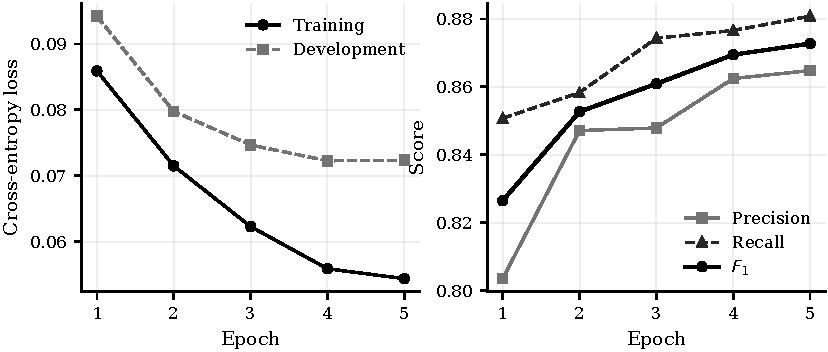
\includegraphics[width=0.92\textwidth]{figures/training_dynamics.pdf}
\caption{Training dynamics over five epochs. Left: loss. Right: development
precision, recall, and $F_1$.}
\Description{Two line charts. The left panel plots training and development cross-entropy loss over five epochs; training loss falls steadily from 0.094 to 0.050 while development loss reaches a minimum of 0.068 at epoch four and rises slightly at epoch five. The right panel plots development precision, recall, and F1 over the same epochs; all three rise monotonically, with F1 improving from 0.80 to 0.85 and recall exceeding precision throughout.}
\label{fig:training}
\end{figure}

\subsection{Per-Type Performance}
\label{sec:nereval:perentity}

Table~\ref{tab:ner_entity} breaks the results down by type and
Figure~\ref{fig:f1_support} plots $F_1$ against support. The relationship is
strong and monotone in the rank sense: Spearman $\rho = 0.75$ ($p = 0.008$),
with Pearson $r = 0.70$ on log-transformed support ($p = 0.016$). Support spans
three orders of magnitude, from 25,839 \texttt{PERSON} instances to 59 for
\texttt{LAW}, and $F_1$ falls from 0.9045 to 0.3514 across that range.

The pattern locates the binding constraint in data volume rather than in model
capacity or linguistic difficulty. Two types sit visibly off the trend and both
are informative. \texttt{WORK\_OF\_ART} reaches 0.8330 on only 284 instances,
far above what its frequency predicts, because titles in this corpus are
dominated by a small set of repeated religious and literary works the model can
effectively memorize. \texttt{PRODUCT} reaches only 0.3514 on 252 instances,
below the trend, because product mentions are lexically open and frequently
share surface form with common nouns.

\begin{table}[htbp]
\centering
\caption{Per-type recognition performance, ordered by $F_1$.}
\label{tab:ner_entity}
\begin{tabular}{lrrrr}
\hline
\textbf{Entity} & \textbf{Precision} & \textbf{Recall} & \textbf{$F_1$} & \textbf{Support} \\
\hline
PERSON        & 0.8893 & 0.9202 & \textbf{0.9045} & 25,839 \\
GPE           & 0.8313 & 0.8604 & 0.8456 &  8,401 \\
WORK\_OF\_ART & 0.8697 & 0.7993 & 0.8330 &    284 \\
ORG           & 0.7533 & 0.8002 & 0.7760 &  8,902 \\
NORP          & 0.7944 & 0.7290 & 0.7603 &  1,860 \\
LANGUAGE      & 0.6638 & 0.8443 & 0.7432 &    456 \\
LAW           & 0.5811 & 0.7288 & 0.6466 &     59 \\
LOC           & 0.6017 & 0.6934 & 0.6443 &    610 \\
FAC           & 0.6167 & 0.5068 & 0.5564 &    219 \\
EVENT         & 0.3654 & 0.5000 & 0.4222 &     76 \\
PRODUCT       & 0.4062 & 0.3095 & 0.3514 &    252 \\
\hline
\end{tabular}
\end{table}

\begin{figure}[htbp]
\centering
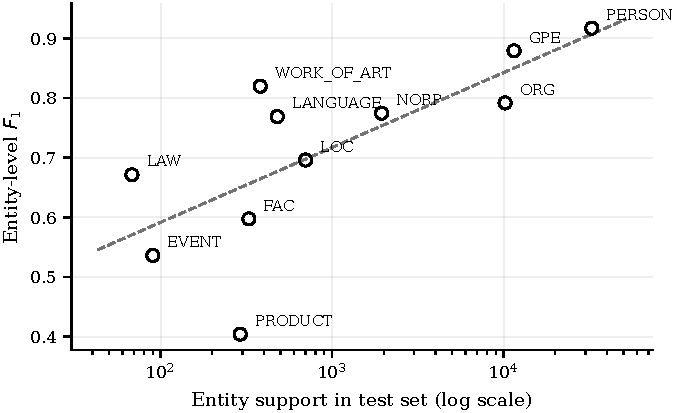
\includegraphics[width=0.70\textwidth]{figures/f1_vs_support.pdf}
\caption{Per-type $F_1$ against test-set support. Dashed line is a
least-squares fit in log support.}
\Description{Scatter plot of per-type F1 against test-set support on a logarithmic horizontal axis, with eleven labeled points and a dashed least-squares trend line. F1 rises with support, from PRODUCT and EVENT below 0.45 at fewer than 300 instances to PERSON at 0.90 with 25,839 instances. WORK OF ART sits well above the trend and PRODUCT well below it.}
\label{fig:f1_support}
\end{figure}

\subsection{Error Structure}
\label{sec:nereval:errors}

Errors cluster among semantically adjacent types rather than scattering, as
Figure~\ref{fig:confusions} shows. The largest single confusion is between
\texttt{GPE} and \texttt{ORG}, with 1,280 \texttt{GPE} tokens labeled
\texttt{ORG} and 628 in the reverse direction. This is the expected consequence
of names denoting both a place and the body that governs it, and the
English-side model makes the same error before projection begins. The next
largest, 961 \texttt{PERSON} tokens labeled \texttt{GPE}, is more specific to
Mizo: many Mizo personal names are formally indistinguishable from place names,
and the sanity-check samples show the projection making exactly this mistake on
names such as \textit{Hminga} and \textit{Liani}.

Since the reference labels are themselves projections, an unknown fraction of
these counted errors are cases where the model is right and the reference is
wrong. Separating the two requires gold annotation.

\begin{figure}[htbp]
\centering
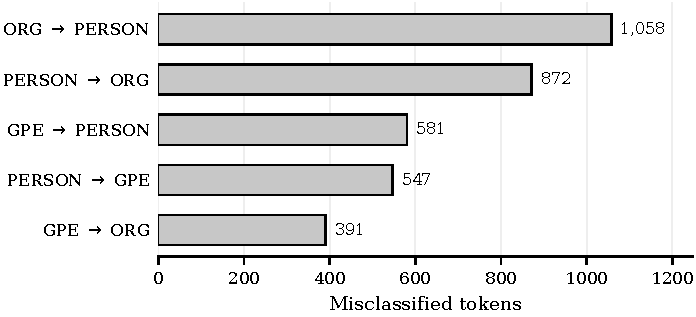
\includegraphics[width=0.62\textwidth]{figures/confusions.pdf}
\caption{Most frequent type confusions on the test set.}
\Description{Horizontal bar chart of the five most frequent entity type confusions. GPE predicted as ORG accounts for 1,280 tokens, PERSON predicted as GPE for 961, ORG predicted as GPE for 628, ORG predicted as NORP for 163, and GPE predicted as LOC for 13.}
\label{fig:confusions}
\end{figure}

%==============================================================================
\section{Entity Markup for Machine Translation}
\label{sec:mt}

\subsection{What This Experiment Measures}
\label{sec:mt:scope}

Named entities are a known weak point in low-resource translation: rare,
frequently out of vocabulary, and prone to omission or mistranslation. Marking
them explicitly in the source may help a translation model preserve them.

This experiment tests that with markup taken from the corrected projection
rather than from the recognizer of Section~\ref{sec:model}. The choice bounds
the interpretation and we state it before reporting any number. A deployed
system has no projection available at inference---it has only the source
sentence and whatever a recognizer predicts, which at micro-$F_1$ 0.8529 will
sometimes be wrong. What follows therefore measures the value of entity markup
under labeling consistent with the training corpus, an upper bound on what a
recognizer-driven pipeline would deliver rather than an estimate of it.

The design has one compensating benefit. Because no recognizer output enters the
translation experiment, there is no possibility that translation gains are
contaminated by the recognizer having seen translation test sentences during its
own training. The two experiments are independent, which the differing split
ratios would otherwise put in doubt.

\subsection{Markup Format}
\label{sec:mt:format}

For a sentence $s$ with projected entities
$\mathcal{E}(s) = \{(e_i, T_i)\}$, the injection operator wraps each span in
type-specific delimiters:

\begin{equation}
\label{eq:inject}
\Phi\bigl(s, \mathcal{E}(s)\bigr) = s',
\qquad
e_i \;\longmapsto\; \texttt{«}T_i\texttt{»}\; e_i \;\texttt{«/}T_i\texttt{»},
\end{equation}

applied in order of decreasing $|e_i|$ so that nested or overlapping matches
resolve to the longest span. Guillemets are used rather than angle brackets
because they do not collide with markup already present in the text. An example:

\begin{quote}
\textbf{Plain:} \textit{Chu chu Fadil-a thil tih a ni.}\\
\textbf{Marked:} \textit{Chu chu} \texttt{«PERSON»} \textit{Fadil} \texttt{«/PERSON»}\textit{-a thil tih a ni.}
\end{quote}

The suffix \textit{-a} falls outside the closing delimiter because the
projection marks the stem, so the translation model sees the entity boundary and
the inflection separately.

\subsection{Systems and Data}
\label{sec:mt:setup}

Two translation systems were trained, identical in every respect except the
source side: a baseline reading plain Mizo, and an augmented system reading
$\Phi(s, \mathcal{E}(s))$. Both target plain English, both start from the same
pretrained checkpoint, and both use the configuration of
Table~\ref{tab:mt_config}.

The 441,178 sentences were split 90/5/5, giving 397,060 training, 22,059
validation, and 22,059 test sentences. Both systems train on the same sentences
and are evaluated on the same test set, so the only difference is the markup.
This split is independent of the 80/10/10 split used for the recognizer.

\begin{table}[htbp]
\centering
\caption{Translation system configuration, identical for both systems.}
\label{tab:mt_config}
\begin{tabular}{ll}
\hline
\textbf{Parameter} & \textbf{Value} \\
\hline
Pretrained model     & \texttt{Helsinki-NLP/opus-mt-mul-en} \citep{tiedemann2020opus} \\
Framework            & MarianMT \citep{junczys2018marian} \\
Parameters           & 77.5M \\
Epochs               & 3 \\
Learning rate        & $5 \times 10^{-5}$ \\
Batch size           & 16, gradient accumulation 4 (effective 64) \\
Weight decay         & 0.01 \\
Warmup steps         & 1,000 \\
Maximum length       & 128 subword tokens \\
Beam width           & 4 \\
Train / valid / test & 397,060 / 22,059 / 22,059 sentences \\
Training time        & 3.98 h (baseline), 8.38 h (marked) \\
\hline
\end{tabular}
\end{table}

\subsection{Metrics and Significance}
\label{sec:mt:metrics}

We report BLEU \citep{papineni2002bleu} and ChrF \citep{popovic2015chrf} as
computed by \texttt{sacrebleu} \citep{post2018sacrebleu}. BLEU is the
brevity-penalized geometric mean of modified $n$-gram precisions,

\begin{equation}
\label{eq:bleu}
\mathrm{BLEU} = \mathrm{BP} \cdot
\exp\left( \sum_{n=1}^{N} w_n \log p_n \right),
\qquad
\mathrm{BP} =
\begin{cases}
1 & \text{if } c > r, \\
e^{\,1 - r/c} & \text{if } c \leq r,
\end{cases}
\end{equation}

with $p_n$ the modified $n$-gram precision, $w_n = 1/N$, $N = 4$, and $c$ and
$r$ the candidate and reference lengths. ChrF is the character $n$-gram
$F_\beta$ score,

\begin{equation}
\label{eq:chrf}
\mathrm{ChrF}_\beta =
(1 + \beta^{2}) \,
\frac{\mathrm{CHRP} \cdot \mathrm{CHRR}}
     {\beta^{2} \cdot \mathrm{CHRP} + \mathrm{CHRR}},
\end{equation}

with $\mathrm{CHRP}$ and $\mathrm{CHRR}$ the character $n$-gram precision and
recall and $\beta = 2$. ChrF matters here because Mizo is morphologically
productive and word-level metrics undercount translations differing only in
inflection.

Significance is assessed by bootstrap resampling \citep{koehn2004significance}.
Drawing $B = 1{,}000$ resamples $\mathcal{S}^{(b)}$ of size $n = 22{,}059$ with
replacement from the test set, we compute the paired difference
$\delta^{(b)} = \mathrm{BLEU}\bigl(\mathcal{S}^{(b)}_{\mathrm{marked}}\bigr) -
\mathrm{BLEU}\bigl(\mathcal{S}^{(b)}_{\mathrm{base}}\bigr)$
and estimate

\begin{equation}
\label{eq:bootstrap}
\hat{p} = \frac{1}{B} \sum_{b=1}^{B} \mathbf{1}\bigl[\delta^{(b)} \leq 0\bigr].
\end{equation}

%==============================================================================
\section{Translation Results}
\label{sec:mtresults}

\subsection{Overall}
\label{sec:mtresults:overall}

Table~\ref{tab:mt_overall} gives the corpus-level scores. Entity markup improves
BLEU by 0.33 and ChrF by 0.24.

\begin{table}[htbp]
\centering
\caption{Corpus-level translation quality on 22,059 test sentences.}
\label{tab:mt_overall}
\begin{tabular}{lrrrr}
\hline
\textbf{System} & \textbf{BLEU} & \textbf{ChrF} & \textbf{$\Delta$BLEU} & \textbf{$\Delta$ChrF} \\
\hline
Baseline (plain source) & 49.74 & 68.19 & --- & --- \\
Entity-marked source    & \textbf{50.06} & \textbf{68.43} & $+0.33$ & $+0.24$ \\
\hline
\end{tabular}
\end{table}

These absolute values should not be compared against Mizo--English results
reported elsewhere. The test set is drawn from the entity-filtered corpus, which
is narrower in domain and denser in entities than general Mizo text, and both
systems were trained on that same restricted distribution. The comparison
between the two rows is meaningful; the rows themselves are not portable.

\subsection{Significance}
\label{sec:mtresults:significance}

Bootstrap resampling under Equation~\eqref{eq:bootstrap} gives a mean BLEU
difference of $+0.331$ with a 95\% confidence interval of $[+0.136, +0.530]$.
The marked system scored higher in 999 of 1,000 resamples and lower in 1, giving
$\hat{p} = 0.001$. The interval lies entirely above zero, so the direction of
the effect is reliable. Its magnitude is small, and the interval is consistent
with anything from roughly a tenth of a BLEU point to half of one.

\subsection{Sentence-Level Outcomes}
\label{sec:mtresults:sentence}

Corpus BLEU hides how the gain is distributed.
Table~\ref{tab:sentence_level} compares the systems sentence by sentence.

\begin{table}[htbp]
\centering
\caption{Sentence-level comparison across the 22,059 test sentences.}
\label{tab:sentence_level}
\begin{tabular}{lrr}
\hline
\textbf{Outcome} & \textbf{Sentences} & \textbf{Share (\%)} \\
\hline
Marked system better & 4,318 & 19.6 \\
Baseline better      & 4,068 & 18.4 \\
No difference        & 13,673 & 62.0 \\
\hline
\end{tabular}
\end{table}

The margin is 250 sentences out of 22,059, a little over one percent of the test
set. Nearly two thirds of sentences are unchanged, and among those that do
change the two systems trade wins almost evenly. The corpus-level gain is the
residue of many small offsetting differences, not a broad improvement. What the
table does establish is that markup is not destabilizing: it causes no
widespread degradation, and the sentences it changes it changes in both
directions at roughly equal rates.

\subsection{By Entity Type}
\label{sec:mtresults:perentity}

Table~\ref{tab:entity_bleu} and Figure~\ref{fig:delta} report BLEU for each
system on the subset of test sentences containing at least one entity of each
type. Sentences containing several types appear in several rows, which is why
the counts sum to more than 22,059.

\begin{table}[htbp]
\centering
\caption{Translation quality on test sentences containing each entity type.
Counts are sentences, not entity instances.}
\label{tab:entity_bleu}
\begin{tabular}{lrrrr}
\hline
\textbf{Entity} & \textbf{Sentences} & \textbf{Baseline} & \textbf{Marked} & \textbf{$\Delta$BLEU} \\
\hline
PERSON        & 13,754 & 52.24 & 52.65 & $+0.41$ \\
GPE           &  5,041 & 49.96 & 50.19 & $+0.23$ \\
ORG           &  4,606 & 49.20 & 49.46 & $+0.27$ \\
NORP          &    927 & 48.42 & 48.65 & $+0.23$ \\
LOC           &    337 & 53.55 & 52.72 & $-0.83$ \\
LANGUAGE      &    246 & 52.21 & 51.67 & $-0.54$ \\
WORK\_OF\_ART &    211 & 37.53 & 38.32 & $+0.79$ \\
FAC           &    178 & 56.46 & 57.71 & $+1.26$ \\
PRODUCT       &    136 & 52.24 & 51.91 & $-0.33$ \\
EVENT         &     35 & 51.53 & 50.44 & $-1.09$ \\
LAW           &     23 & 57.64 & 58.65 & $+1.02$ \\
\hline
\end{tabular}
\end{table}

\begin{figure}[htbp]
\centering
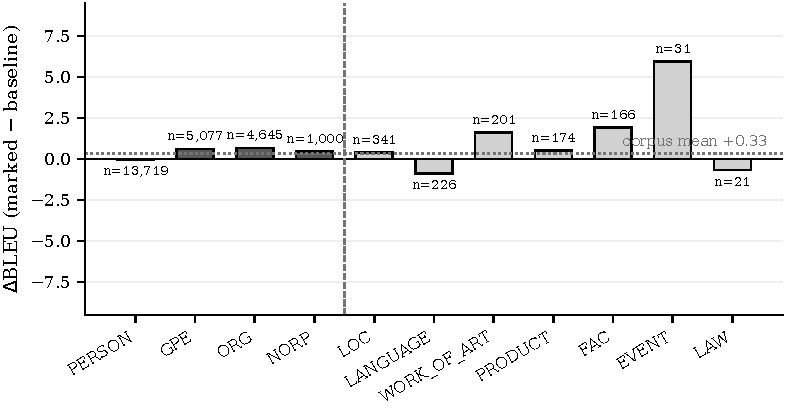
\includegraphics[width=0.88\textwidth]{figures/per_entity_delta.pdf}
\caption{Per-type BLEU difference, ordered by sentence count. Dotted line marks
the corpus-level mean.}
\Description{Bar chart of per-type BLEU difference between the entity-marked and baseline translation systems, ordered by decreasing sentence count and annotated with those counts. The four frequent types on the left, shown in dark bars, all show small positive differences between plus 0.23 and plus 0.41, close to the corpus mean of plus 0.33 marked by a dotted line. The seven sparse types on the right, shown in light bars, scatter widely in both directions from minus 1.09 to plus 1.26.}
\label{fig:delta}
\end{figure}

The four most frequent types---\texttt{PERSON}, \texttt{GPE}, \texttt{ORG}, and
\texttt{NORP}, covering 24,328 of the 25,494 sentence-type pairs---all show
small positive differences between $+0.23$ and $+0.41$. These are the only
estimates in the table with enough support to be stable, and they agree with
each other and with the corpus-level figure.

The larger numbers in both directions all belong to the sparsest types:
\texttt{FAC} at $+1.26$ on 178 sentences, \texttt{EVENT} at $-1.09$ on 35,
\texttt{LAW} at $+1.02$ on 23. Differences of this size on samples of this size
are what sampling variation produces. We draw no conclusion about whether markup
helps or harms any particular entity type, and we would caution against reading
the sign of any row below \texttt{NORP}. Reporting them is a matter of
completeness, not evidence.

%==============================================================================
\section{Discussion}
\label{sec:discussion}

\subsection{What Projection Delivered, and What It Did Not}
\label{sec:discussion:projection}

The headline number for the method is not the corpus size but the recovery rate
of Table~\ref{tab:projection_recovery}. Exact matching found 4\% of English
entities in the aligned Mizo text. The reason is exactly the morphology of
Section~\ref{sec:mizo}: Mizo attaches case suffixes to proper nouns as a matter
of course, so the surface form in the Mizo sentence rarely matches the English
one. Adding suffix stripping raised recovery tenfold. For languages with this
profile, the morphological component is not an optimization but the thing that
makes projection work at all, and we would encourage other projection work on
morphologically rich targets to report the comparison rather than only the final
corpus size.

Recovery nonetheless stops below 42\%, so the majority of English entities never
reach the Mizo side. Recall is where the neural projection methods of
Section~\ref{sec:related:projection} would help once the models they require
exist for Mizo.

The correction process deserves precision. Eight rounds of inspecting random
samples and generalizing errors into rules is a real human-in-the-loop procedure
and it corrected 100,237 labels. It is not verification. Inspection of the final
rounds still turns up errors---personal names labeled \texttt{GPE}, ethnonyms
labeled \texttt{PERSON}, football clubs labeled \texttt{FAC}. Residual label
noise remains at a rate we have not measured, and any user of the corpus should
plan around that.

\subsection{Transfer Without Pretraining}
\label{sec:discussion:transfer}

XLM-RoBERTa reaches micro-$F_1$ 0.8529 on a language it never saw. The plausible
mechanism is subword overlap: Mizo uses the Latin script and its character
$n$-gram inventory intersects substantially with languages the model did see.
Mizo's regular suffixation may also help, letting the model associate inflected
and bare forms of the same name from repeated exposure.

We flag this as a plausible account rather than a demonstrated one. Establishing
it would require ablations we did not run---against mBERT, against zero-shot
XLM-RoBERTa without fine-tuning, against a model trained from scratch, and now
against MizBERT \citep{lalramhluna2024mizbert}. Without those, the contribution
of pretraining cannot be separated from the contribution of 352,941 training
sentences.

\subsection{The Size of the Translation Effect}
\label{sec:discussion:mteffect}

The translation result is best stated conservatively. Entity markup produces a
gain consistent in direction across bootstrap resamples and small in
magnitude---about a third of a BLEU point---under conditions more favorable than
a deployed system would face. The sentence-level breakdown shows the mechanism
is not a broad lift but a narrow net advantage over many offsetting changes.

This is still worth reporting. Low-resource translation offers few interventions
that reliably improve anything, and one that costs nothing at the architecture
level and does no measurable harm has practical value. But it does not support a
claim that entity information substantially improves Mizo--English translation,
and we do not make one.

The obvious next experiment is the one we did not run: substitute recognizer
predictions for projection labels at test time and measure the drop. The gap is
the price of the pipeline, and for a recognizer at micro-$F_1$ 0.85 it may
consume the entire gain. Reporting that number, positive or negative, would be a
useful contribution in itself.

\subsection{Calibrating Silver Against Gold}
\label{sec:discussion:calibration}

Every figure in Sections~\ref{sec:nereval} and~\ref{sec:mtresults} is an
agreement statistic against projection labels. The natural next step is
calibration against the gold Mizo annotations now available
\citep{ghosh2025mizokhasi}: evaluating our recognizer on a gold test set would
convert every number here into an accuracy, and comparing a model trained on our
441,178 silver sentences against one trained on gold data would establish
directly what the size-quality trade buys. Differences in annotation guidelines
and entity inventory would need reconciling first, which is why we flag this as
future work rather than reporting it.

%==============================================================================
\section{Limitations}
\label{sec:limitations}

\paragraph{Silver-standard evaluation.}
Every label, training and test alike, comes from the same projection pipeline.
The reported $F_1$ measures agreement with the projection, not accuracy against
human annotation, and the true accuracy is unknown and likely lower. This is the
principal limitation of the work.

\paragraph{Entity markup, not recognizer output.}
The translation experiment uses markup from the corrected projection. The
corresponding pipeline figure, using recognizer predictions, has not been
measured and would be lower.

\paragraph{Missing baselines.}
We did not compare against mBERT, zero-shot XLM-RoBERTa, a CRF or BiLSTM
baseline, or MizBERT \citep{lalramhluna2024mizbert}. The last is the most
consequential omission, since a Mizo-specific encoder is the natural competitor
to a multilingual one on this task.

\paragraph{No comparison against gold Mizo data.}
We do not evaluate on the gold Mizo entity data of \citet{ghosh2025mizokhasi},
nor compare a silver-trained model against a gold-trained one. Until that is
done, the size-quality trade this paper takes is argued rather than demonstrated.

\paragraph{Projection recall.}
Recovery reaches 41.91\% on the held-out subset. Entities whose Mizo realization
diverges beyond the covered suffixes---phonologically adapted borrowings, native
translations of English names---are missed systematically rather than at random,
which may bias the corpus toward entity types that transfer as surface strings.

\paragraph{Selection effect from filtering.}
Retaining only entity-bearing sentences makes the corpus denser in entities than
running Mizo text. Both the recognizer and the translation systems were trained
and evaluated on this distribution, so performance on entity-sparse text is
untested.

\paragraph{Single direction, automatic metrics only.}
Translation is evaluated Mizo-to-English with BLEU and ChrF. Whether entity
names are correctly rendered is precisely what markup is meant to address, and
answering it requires human evaluation of entity fidelity.

\paragraph{Domain of the English tagger.}
\texttt{en\_core\_web\_sm} is trained on OntoNotes, whose domains do not match
the parallel corpus used here. Errors in English-side detection propagate
through projection, and the \texttt{GPE}/\texttt{ORG} confusion of
Section~\ref{sec:nereval:errors} is visible in the English annotations before
projection begins.

%==============================================================================
\section{Ethical Considerations}
\label{sec:ethics}

This work creates language resources for a community poorly served by existing
tools, which we believe is broadly beneficial for access to information and for
documentation. The corpus derives from a Mizo--English parallel corpus assembled
from published and publicly circulated text, and no personal information beyond
what those sources already contain has been introduced.

Entity recognition can also support surveillance and profiling, and this risk is
sharper for minority-language communities, who are more often the subject of
such systems than the beneficiaries of them. We ask users of these resources to
weigh that in their applications.

%==============================================================================
\section{Conclusion}
\label{sec:conclusion}

We have presented a silver-standard Mizo entity corpus of 441,178 sentences and
590,655 annotations, built by projecting English entities across a
Mizo--English parallel corpus with a morphology-aware matcher that raises entity
recovery from 4.14\% to 41.91\% by accommodating Mizo's productive case marking,
followed by eight rounds of sample-driven rule correction. Fine-tuned
XLM-RoBERTa reaches 97.84\% token accuracy and micro-$F_1$ 0.8529 across eleven
types on a language absent from its pretraining, with per-type performance
tracking annotation frequency closely enough to place the constraint on data
rather than architecture. Inserting entity markup into the source side of a
Mizo-to-English translation system yields $+0.33$ BLEU and $+0.24$ ChrF,
reliable in direction and modest in size, measured under conditions that bound
from above what a recognizer-driven pipeline would achieve.

The resource complements rather than replaces the gold Mizo annotations that
have recently become available: it trades label quality for three orders of
magnitude in scale, and the most valuable next step is to measure that trade
directly by calibrating against gold data. Beyond that, richer projection
methods would address the recall ceiling, a Mizo-specific encoder is the obvious
missing baseline, and human evaluation of entity fidelity would test the
translation claim on the terms that matter.

%==============================================================================
\begin{acks}
The authors thank the Head, Department of Mathematics and Computer Science, and
the Dean, School of Physical Sciences, Mizoram University, for institutional
support.
% TODO: add funding acknowledgment if applicable.
\end{acks}

%==============================================================================
\bibliographystyle{ACM-Reference-Format}
\bibliography{refs}

\end{document}
